\documentclass{template}
\usepackage[english]{babel}

\begin{document}
% New Macros for Title, author, date
\newcommand{\mytitle}{Mathematics II}
\newcommand{\CourseCode}{Eng Tech 1MT3}
\newcommand{\myauthor}{Aaron Chiu}
\newcommand{\mydate}{\today}

\begin{titlepage}
\begin{center}
    \Large \mytitle \\
    \large \myauthor \\
    \mydate

\end{center}
\end{titlepage}

\tableofcontents

% HEADER & FOOTER
\lhead{\mytitle}
\rhead{\nouppercase{\leftmark}}
\cfoot{\thepage}
\raggedright

% Content Beginning
\newpage
\section{Pre - Integration}
\subsection{Riemann Sums} % Riemann Sums
The area under a curve can be split into multiple different rectangles. Adding the rectangles results in the total area.
\begin{align*}
    y = f(x); \ a \leq x \leq b; \ \text{with $n$ sub intervals}
\end{align*}

\begin{mdframed_title}{Using Left Endpoints}
    \begin{align*}
        R_l = \sum_{i = 1}^n f(x_i) \Delta x && x_i=a+i \Delta x -  \Delta x && \Delta x = \frac{b - a}{n}
    \end{align*}
\end{mdframed_title}

\begin{mdframed_title}{Using Right Endpoints}
    \begin{align*}
        R_r = \sum_{i = 1}^n f(x_i) \Delta x && x_i=a+i \Delta x && \Delta x = \frac{b - a}{n}
    \end{align*}
\end{mdframed_title}

\begin{mdframed_title}{Using Midpoints (Average)}
    \begin{align*}
        R_m = \sum_{i = 1}^n f(\bar{x_i}) \Delta x && \bar{x_i}=a+i \Delta x -\frac{1}{2} \Delta x && \Delta x = \frac{b - a}{n}
    \end{align*}
\end{mdframed_title}

When $n$ is small, this results in areas that are not taken into account resulting in an inaccurate area.

\subsection{Definite Integral}
When there are an infinitesimal amount of sub intervals, this results in the actual area under the curve.
\begin{align*}
    \lim_{n\to\infty}\sum_{i = 1}^n f(x_i^*) = \int_a^b f(x)dx
\end{align*}
Where $\int_a^b f(x)dx$ is the definite integral of the functions running from a to b.



\newpage
\section{Fundamental Theorems of Calculus (FTC)}
\subsection{Part 1} % Part 1 FTC
\begin{mdframed}
    \begin{align*}
        \text{If: } g(x) = \int_a^x f(t) dt && \text{Then: } g'(x) = f(x)
    \end{align*}
    $$ \text{Alternatively: } \frac{d}{dx}\int_a^x f(t) dt = f(x) $$
\end{mdframed}

Take note that the upper limit is in the form of $\int_a^x f(t) dt$ and not any other form.

\vspace{4 mm}
\begin{tcolorbox}
\textbf{Example:} Evaluate: $ \displaystyle g'(x) = \int_a^{x^2} \sin(t) dt$ \\
Due to the the integral not being the form of $\int_a^x f(t) dt$, we need to do a substitution.

\begin{align*}
    g(x) &= \int_a^{x^2} \sin(t) dt & u &= x^2 \\
    g(x) &= \int_a^u \sin(t) dt & \\
    g'(u) &= \sin(u) &
\end{align*}

We need to undo our substitution, however cannot directly undo it. Therefore, we will need to use the chain rule.

\begin{align*}
    \frac{dg}{du} &= \sin(u) & \\
    \frac{dg}{dx}\frac{dx}{du} &= \sin(u) & \\
    \frac{dg}{dx} &= \sin(u) \ \frac{du}{dx} & du &= 2x \ dx
\end{align*}

\begin{empheq}[box=\fbox]{align*}
    \frac{dg}{dx} &= \sin(x^2) \ 2x
\end{empheq}
\end{tcolorbox}

\newpage
\subsection{Part 2} % Part 2 FTC
\begin{mdframed}
    $$\int_a^b f(x) \ dx = F(b) - F(a)$$
    \center{Where $F$ is the anti derivative (integral) of $f$}
\end{mdframed}

\textbf{Applications} \\
If a particle is defined by a speed of $v(x)$, Then the displacement and speed through the time $a \leq t \leq b$ are:
\begin{align*}
    \Vec{d} \ \text{(Displacement)} &= \int_a^b v(t) \ dt \\
    \text{$d$ (Distance)} &= \int_a^b |v(t)| \ dt
\end{align*}

\section{Integration Techniques}
\subsection{Integration by Substitution} % Substitution

\begin{mdframed}
    \begin{align*}
        \int f(g(x) \ g'(x) = \int f(u) \ du && \text{Where } u = g(x)
    \end{align*}
\end{mdframed}

\textbf{Indefinite Integrals} need to have their substitution undone 

\vspace{4 mm}
\begin{tcolorbox}
\textbf{Example:} Evaluate: $\displaystyle \int \frac{x+3}{\sqrt{x^2 + 6x}} \ dx$ \\
We'll have to do a substitution for $x^2 + 6x$ as we don't know the integral of a function in a radical
\begin{align*}
    &\phantom{{}={}} \int \frac{x+3}{\sqrt{x^2 + 6x}} \ dx & u &= x^2 + 6x \\
    &= \int \frac{1}{2} \frac{du}{\sqrt{u}} & du &= (2x + 6) \ dx \\
    &= \frac{1}{2}\int u^{-\tfrac{1}{2}} \ du & \frac{1}{2} \ du &= (x + 3) \ dx \\
    &= \frac{1}{2}(\frac{u^{\tfrac{1}{2}}}{\tfrac{1}{2}}) + C & \\
    &= u^{\tfrac{1}{2}} + C & \\
    &= (x^2 + 6x)^{\tfrac{1}{2}} + C &
\end{align*}
\end{tcolorbox}

\begin{itemize}
    \item Remember to substitute for $dx$ as well
    \item You have to replace all occurrences of the original variables (No mixing of variables)
\end{itemize}

\textbf{Definite Integrals} need to have their bounds changed

\vspace{3 mm}
\begin{tcolorbox}
\textbf{Example:} Evaluate: $\displaystyle \int_0^2 \frac{x+3}{\sqrt{x^2 + 6x}} \ dx$ \\
We've already done this integral from the last example. However, this time, it is a definite integral.

\begin{align*}
    \int_0^2 \frac{x+3}{\sqrt{x^2 + 6x}} \ dx && u = x^2 + 6x && \frac{1}{2} \ du &= (x + 3) \ dx
\end{align*}

We must change the bounds of the integral using $u = x^2 + 6x$.

\begin{center}
    \begin{tabular}{c|c}
        x & u \\ \hline	
        0 & 0 \\
        2 & 16
    \end{tabular}
\end{center}

\begin{align*}
    &\phantom{{}={}} \frac{1}{2}\int_0^{16} \frac{du}{\sqrt{u}} \ dx \\
    &= u^{\tfrac{1}{2}}\big|_0^{16} \\
    &= 16^{\tfrac{1}{2}}-0^{\tfrac{1}{2}} \\
    &= 4
\end{align*}
\end{tcolorbox}

\subsection{Integration of Symmetric Functions}
\begin{mdframed}
    \begin{align*}
        &\text{If $f$ is an even function, then $\int_{-a}^a f(x) \ dx = 2\int_0^a f(x) \ dx$} \\
        &\text{If $f$ is an odd function, then $\int_{-a}^a f(x) \ dx = 0$}
    \end{align*}
\end{mdframed}

\newpage
\subsection{Integration by Parts} % Parts
\begin{mdframed}
    \begin{align*}
        \int u \ dv = uv - \int v \ du && \text{If $u = f(x)$ and $v = g(x)$}
    \end{align*}
    $$ \text{Alternatively: } \int uv = u \int \bigg[v\bigg] - \int \bigg[du \int v\bigg] $$
\end{mdframed}

\vspace{3 mm}
\begin{tcolorbox}
\textbf{Example:} Find the integral of: $\displaystyle \int e^x\cos{2x} \ dx$ \\
Determine what should be $u$ and what should $dv$:
\begin{align*}
    u &= e^x & dv &= \cos{2x} \ dx \\
    du &= e^x \ dx & v &= \frac{\sin{2x}}{2}
\end{align*}
\begin{align*}
    &\phantom{{}={}} e^x \ \frac{\sin{2x}}{2} - \int \frac{\sin{2x}}{2} \ e^x \ dx \\
    &= \frac{1}{2} \ e^x\sin{2x} - \frac{1}{2} \int \sin{2x} \ e^x \ dx
\end{align*}

We must do integration by parts once again.
\begin{align*}
    u &= e^x & dv &= \sin{2x} \ dx \\
    du &= e^x \ dx & v &= -\frac{\cos{2x}}{2}
\end{align*}
\begin{align*}
    &\phantom{{}={}} \frac{1}{2} \ e^x\sin{2x} - \frac{1}{2} \bigg(e^x \cdot -\frac{\cos{2x}}{2} - \int -\frac{\cos{2x}}{2} \ e^x \ dx \bigg) \\
    &= \frac{1}{2} \ e^x\sin{2x} + \frac{1}{4} \ e^x \cos{2x} + \frac{1}{4} \int \cos{2x} \ e^x \ dx
\end{align*}
We have the original integral so we are now in a position to subtract both side by it.
\begin{align*}
    \frac{3}{4} \int e^x\cos{2x} \ dx &= \frac{1}{2} \ e^x\sin{2x} + \frac{1}{4} \ e^x \cos{2x} \\
    \int e^x\cos{2x} \ dx &= \frac{4}{3} \bigg(\frac{1}{2} \ e^x\sin{2x} + \frac{1}{4} \ e^x \cos{2x}\bigg)
\end{align*}
\begin{empheq}[box=\fbox]{align*}
    \frac{2}{3} \ e^x\sin{2x} + \frac{1}{3} \ e^x \cos{2x}
\end{empheq}
\end{tcolorbox}

\subsection{Trigonometric Integrals}
If in the form of $\displaystyle\int \sin^m x\cos^n x \ dx$
\begin{mdframed_title}{Odd Cosine Powers}
    Using the identity $\cos^2 x = 1 - \sin^2 x$
    \begin{align*}
        \int \sin^m x\cos^{2k+1} x \ dx &= \int \sin^m x(\cos^2 x)^k \cos{x} \ dx \\
        &= \int \sin^m x(1-\sin^2 x)^k x \cos{x} \ dx 
    \end{align*}
    Then substitute $u = \sin{x}$
\end{mdframed_title}
\begin{mdframed_title}{Odd Sine Powers}
    Using the identity $\sin^2 x = 1 - \cos^2 x$
    \begin{align*}
        \int \sin^{2k+1} x\cos^n x \ dx &= \int (\sin^2 x)^k \cos^n x \sin{x} \ dx \\
        &= \int (1-\cos^2 x)^k \cos^n x \sin{x} \ dx 
    \end{align*}
    Then substitute $u = \cos{x}$
\end{mdframed_title}
\begin{mdframed_title}{Both Even Sine \& Cosine Powers}
    These can be reduced using the following identities
    \begin{align*}
        \sin^2 x = \frac{1}{2}(1 - \cos 2x) && \cos^2 x = \frac{1}{2}(1 + \cos 2x)
    \end{align*}
    $$\sin x \cos x = \frac{1}{2} \sin 2x$$
\end{mdframed_title}

If in the form of (1) $\displaystyle\int \sin mx \ \cos nx \ dx$, (2) $\displaystyle\int \sin mx \ \sin nx \ dx$, or (3) $\displaystyle\int \cos mx \ \cos nx \ dx$

\begin{mdframed}
    \begin{align}
        \sin A \ \cos B &= \frac{1}{2} [\sin(A-B)+\sin(A+B)] \\
        \sin A \ \sin B &= \frac{1}{2} [\cos(A-B)-\cos(A+B)] \\
        \cos A \ \cos B &= \frac{1}{2} [\cos(A-B)+\cos(A+B)]
    \end{align}
\end{mdframed}

\newpage
If in the form of $\displaystyle\int \tan^m x\sec^n x \ dx$
\begin{mdframed_title}{Even Secant Powers}
    Using the identity $\sec^2 x = 1 + \tan^2 x$
    \begin{align*}
        \int \tan^m x\sec^{2k} x \ dx &= \int \tan^m x(\sec^2 x)^{k-1} \sec^2 x \ dx \\
        &= \int \tan^m x(1+\tan^2 x)^{k-1} \sec{x} \ dx 
    \end{align*}
    Then substitute $u = \tan{x}$
\end{mdframed_title}

\begin{mdframed_title}{Odd Tangent Powers}
    Using the identity $\tan^2 x = \sec^2 x - 1$
    \begin{align*}
        \int \tan^{2k+1} x\sec^n x \ dx &= \int (\tan^2 x)^k \sec^{n-1} x \sec x \tan x\ dx \\
        &= \int (\sec^2 x-1)^k \sec^{n-1} x \sec x \tan x\ dx 
    \end{align*}
    Then substitute $u = \sec{x}$
\end{mdframed_title}

\begin{mdframed_title}{Odd Secant \& Even Tangent}
    The only way to solve these is to use integration by parts
\end{mdframed_title}

\vspace{3 mm}
\begin{tcolorbox}
\textbf{Example:} Evaluate: $\displaystyle \int \sin^5 x \cos^2x \ dx$ \\
Since the power of sin is odd we will have to substitute $u = \cos x$ after some manipulation to get it into the right form

\begin{align*}
    &= \int \sin^4 x \cos^2 x \sin x \ dx       & u &= \cos x\\
    &= \int (1-\cos^2 x)^2 \cos^2 x \sin x \ dx & du &= -\sin x \ dx\\
    &= -\int (1 - u^2)^2 \ u^2 \ du                & -du &= \sin x \ dx \\
    &= -\int (1 - 2u^2 + u^4) \ u^2 \ du \\
    &= -\int (u^2 - 2u^4 + u^6) \ du \\
    &= -(\frac{1}{3} u^3 - \frac{2}{5} u^5 + \frac{1}{7} u^7) + C
\end{align*}

\begin{empheq}[box=\fbox]{align*}
    -\frac{1}{3} \cos^3 x + \frac{2}{5} \cos^5 x - \frac{1}{7} \cos^7 x + C
\end{empheq}
\end{tcolorbox}

\subsection{Trigonometric Substitution} % Trig Sub
For when the integral contains $\sqrt{a^2+x^2}$ or similar comes up.

\begin{mdframed_title}{Table of Different Forms and Their Substitution}
\begin{center}
    \newcolumntype{C}[1]{>{\centering\arraybackslash}p{#1}}
    \renewcommand{\arraystretch}{1.9}
        \begin{tabular}{C{48 mm}|C{48 mm}|C{48 mm}}
        \text{Form} & \text{Substitution} & \text{Identity} \\ \hline
        $\displaystyle \sqrt{a^2-x^2}$ & $\displaystyle x=a\sin \theta$ & $\displaystyle 1-\sin^2\theta=\cos^2\theta$ \\
        $\displaystyle \sqrt{a^2+x^2}$ & $\displaystyle x=a\tan \theta$ & $\displaystyle 1+\tan^2\theta=\sec^2\theta$ \\
        $\displaystyle \sqrt{x^2-a^2}$ & $\displaystyle x=a\sec \theta$ & $\displaystyle \sec^2\theta-1=\tan^2\theta$ \\
        \end{tabular}
    \renewcommand{\arraystretch}{1}    
\end{center}
\end{mdframed_title}

\vspace{3 mm}
\begin{tcolorbox} [breakable, enhanced]
\textbf{Example:} Evaluate: $\displaystyle \int \frac{\sqrt{16-x^2}}{x^2} \ dx$ \\
We can immediate recognise that the radical is in the form of $\sqrt{a^2-x^2}$ so therefore, we will substitute $x=a\sin\theta$
\begin{align*}
    &\phantom{{}={}} \sqrt{4^2-x^2} & x&=4\sin\theta\\
    &= \sqrt{4^2-(4\sin\theta)^2} & dx&=4\cos\theta \ d\theta \\
    &= \sqrt{4^2(1-\sin^2\theta)} & \\
    &= 4\sqrt{\cos^2\theta} & \\
    &= 4\cos\theta &
\end{align*}

Substitute back into the the original equation.

\begin{align*}
    &\phantom{{}={}} \int \frac{4\cos\theta}{(4\sin\theta)^2} \ 4\cos\theta \ d\theta \\
    &= \int \frac{16\cos^2\theta}{16\sin^2\theta} \ d\theta \\
    &= \int \cot^2\theta \ d\theta \\
    &= \int (\csc^2\theta - 1)\ d\theta \\
    &= -\cot\theta - \theta + C
\end{align*}

\newpage
We have to undo our substitution turning $\theta$ back into $x$. We can use a right triangle to help.

\begin{center}
    \(\begin{aligned}
    x &= 4\sin\theta \\
    \frac{x}{4} &= \sin\theta
    \end{aligned}\)\qquad \qquad
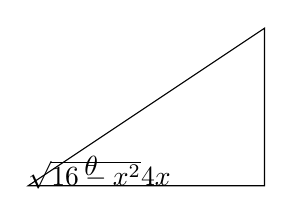
\begin{tikzpicture}[baseline=4ex]
\coordinate [label={[shift={(8 mm, 0.09 mm)}]$\theta$}] (A) at (0,0);
\coordinate (B) at (3,0);
\coordinate (C) at (3,2);

\draw (A)--(B)--(C)--cycle;

\tkzLabelSegment[below=2pt](A,B){\textit{$\sqrt{16-x^2}$}}
\tkzLabelSegment[right=2pt](B,C){\textit{$4$}}
\tkzLabelSegment[above left=2pt](A,C){\textit{$x$}}

\draw (2.75,0) -- (2.75,0.25) -- (3, 0.25);
\end{tikzpicture}

\end{center}

\begin{empheq}[box=\fbox]{align*}
    -\frac{\sqrt{16-x^2}}{4} - \arcsin\frac{x}{4} + C
\end{empheq}
\end{tcolorbox}

\subsection{Integration by Partial Fraction Decomposition}
These come in the form of $\displaystyle f(x)=\frac{P(x)}{Q(x)}$ where both $P(x)$ and $Q(x)$ are polynomials

\textbf{Step 1}
\begin{itemize}
    \item If the degree of $P<Q$ then this is called \textbf{Proper} and we can move onto the next step
    \item If the degree of $P\geq Q$ then this is called \textbf{Improper} and we must reduce it to a proper fraction using either long or short division to obtain a function in the form of:
\end{itemize}
$$f(x)=\frac{P(x)}{Q(x)}=S(x)+\frac{R(x)}{Q(x)}$$

\textbf{Step 2} \\
Reduce the denominator $Q(x)$ into either linear or irreducible quadratic factors:
$$ax+b \quad \text{or} \quad ax^2+bx+c \ \text{where} \ b^2-4ac<0$$

\textbf{Step 3 (Denominator)}\\
We can split the the whole function into forms of either:
$$\frac{A}{ax+b} \quad \text{or} \quad \frac{Ax+B}{ax^2+bx+c}$$

\textbf{Case 1: } We can express $Q(x)$ as a product of linear factors
$$\frac{R(x)}{Q(x)}=\sum_{i=1}^n\frac{A_i}{a_ix+b_i}$$

\textbf{Case 2: } We can express $Q(x)$ as a product of linear factors where some a repeated  (Where $a_ix+b_i$ is repeated $r$ times)
$$\frac{A_1}{a_ix+b_i}+\frac{A_i}{(a_ix+b_i)^2}+\dots+\frac{A_i}{(a_ix+b_i)^r}$$

\textbf{Case 3: } We can express $Q(x)$ as a product of linear factors and quadratic factors
$$\frac{A_ix+B}{a_ix^2+b_ix+c_i}$$

\textbf{Case 4: } We can express $Q(x)$ as a product of linear factors and quadratic factors where some a repeated (Where $a_ix^2+b_ix+c_i$ is repeated $r$ times)
$$\frac{A_ix+B}{a_ix^2+b_ix+c_i}+\frac{A_ix+B}{(a_ix^2+b_ix+c_i)^2}+\dots+\frac{A_ix+B}{(a_ix^2+b_ix+c_i)^r}$$
These terms can be integrated by substitution and \textbf{completing the square.}

\vspace{3 mm}
\textbf{Step 3 (Numerator)}
To determine the coefficients given $\displaystyle\frac{R(x)}{Q(x)}$ follow this procedure.

\begin{align*}
    \frac{R(x)}{Q(x)}&=\sum_{i=1}^n\frac{A_i}{a_ix+b_i} \\
    R(x)&=\sum_{i=1}^n A_i \ \frac{Q(x)}{a_ix+b_i}
\end{align*}

After dividing, distribute $A_i$, and then collect like terms in a matrix from and solve for the coefficients. We can also set $x$ in a way that makes the other factors 0.

\vspace{3 mm}
\begin{tcolorbox} [breakable, enhanced]
\textbf{Example:} Evaluate: $\displaystyle \int \frac{7x^2-5x+6}{x^3-10x^2+21x} \ dx$ \\
The first step is to factor the denominator and then split into different fractions with numerators undetermined for now.
$$\frac{7x^2-5x+6}{x(x-3)(x-7)} = \frac{A}{x}+\frac{B}{x-3}+\frac{C}{x-7}$$

Multiply by the original (factored) denominator
\begin{align*}
    &\phantom{{}={}}\frac{A}{x} \ x(x-3)(x-7) & &\phantom{{}={}}\frac{B}{x-3} \ x(x-3)(x-7) & &\phantom{{}={}}\frac{C}{x-7} \ x(x-3)(x-7) \\
    &= A(x-3)(x-7) & &= Bx(x-7) & &= Cx(x-3)
\end{align*}

Set them equal to the denominator
$$7x^2-5x+6=A(x-3)(x-7) + Bx(x-7) + Cx(x-3)$$

Solve for the coefficients by letting $x=0,3,7$
\begin{align*}
    x&=0 & 7(0)^2-5(0)+6 &= A[(0)-3][(0)-7] & A&= \frac{2}{7} \\
    x&=3 & 7(3)^2-5(3)+6 &= B(3)[(3)-7]     & B&= -\frac{9}{2} \\
    x&=7 & 7(7)^2-5(7)+ 6&= C(7)[(7)-3]     & C&= \frac{157}{14} \\
\end{align*}

\newpage
We can now go back to the original integral

$$\int \frac{7x^2-5x+6}{x^3-10x^2+21x} \ dx = \frac{2}{7} \int \frac{dx}{x} -\frac{9}{2}\int\frac{dx}{x-3} +\frac{157}{14}\int\frac{dx}{x-7}$$

\begin{empheq}[box=\fbox]{align*}
    \frac{2}{7}\ln|x|-\frac{9}{2}\ln|x-3|+\frac{157}{14}\ln|x-7|+C
\end{empheq}
\end{tcolorbox}

\vspace{3 mm}
\begin{tcolorbox} [breakable, enhanced]
\textbf{Example:} Evaluate: $\displaystyle \int \frac{4x^2+5x+2}{4x^2+4x+3} \ dx$ \\
Since the degree of the numerator is greater or equal to the denominator, we must first use long division
\begin{center}
    \polylongdiv{4x^2+5x+2}{4x^2+4x+3}
\end{center}

\begin{align*}
    \frac{4x^2+5x+2}{4x^2+4x+3}=1+\frac{x-1}{4x^2+4x+3} && \int 1 dx = x
\end{align*}

Complete the square of the denominator
\begin{align*}
    4x^2+4x+3 &= 4\bigg(x^2+x+\frac{3}{4}\bigg) \\
              &= 4\bigg(x^2+x+\bigg(\frac{1}{2}\bigg)^2-\bigg(\frac{1}{2}\bigg)^2+\frac{3}{4}\bigg) \\
              &= 4\bigg(x+\frac{1}{2}\bigg)^2+2
\end{align*}

Make the substitution of the square (ie $\displaystyle u=x+\frac{1}{2}$)

\begin{align*}
    &\phantom{{}={}}\int\frac{x-1}{4x^2+4x+3} \ dx & u &= x+\frac{1}{2} \\
    &= \int\frac{u-\frac{1}{2}-1}{4u^2+2} \ du     & du &= dx \\
    &= \int\frac{u-\frac{3}{2}}{4u^2+2}  \ du      & x &= u-\frac{1}{2}
\end{align*}

Now it is in a form we can work with
\begin{align*}
    \frac{u-\frac{3}{2}}{4u^2+2} &= \frac{u}{4u^2+2} - \frac{\frac{3}{2}}{4u^2+2}\\
\end{align*}

Take the integral for what we have now, using what techniques we know
\begin{align*}
    &\phantom{{}={}}\frac{1}{2}\int\frac{u}{2u^2+1} \ du- \frac{3}{4}\int\frac{1}{2u^2+1} \ du\\
    &= \frac{1}{2} \ \frac{1}{4} \ln|2u^2+1|-\frac{3}{8} \ \frac{1}{\sqrt{2}}\arctan (\sqrt{2}u) + C
\end{align*}

Substitute back in what we have
\begin{empheq}[box=\fbox]{align*}
   x+\frac{1}{8} \ln|2(x+\frac{1}{2})^2+1|-\frac{3}{8\sqrt{2}} \arctan (\sqrt{2}(x+\frac{1}{2})) + C
\end{empheq}
\end{tcolorbox}

\section{Applications of Integration}









\end{document}